%
% File emnlp2020.tex
%
%% Based on the style files for ACL 2020, which were
%% Based on the style files for ACL 2018, NAACL 2018/19, which were
%% Based on the style files for ACL-2015, with some improvements
%% taken from the NAACL-2016 style
%% Based on the style files for ACL-2014, which were, in turn,
%% based on ACL-2013, ACL-2012, ACL-2011, ACL-2010, ACL-IJCNLP-2009,
%% EACL-2009, IJCNLP-2008...
%% Based on the style files for EACL 2006 by 
%%e.agirre@ehu.es or Sergi.Balari@uab.es
%% and that of ACL 08 by Joakim Nivre and Noah Smith

\documentclass[11pt,a4paper]{article}
\usepackage[hyperref]{emnlp2020}
\usepackage{times}
\usepackage{latexsym}
\usepackage{graphicx}
\usepackage{amssymb}
\usepackage{natbib}
\usepackage{epstopdf} %%package to overcome problem with eps in pdf files
\renewcommand{\UrlFont}{\ttfamily\small}

% This is not strictly necessary, and may be commented out,
% but it will improve the layout of the manuscript,
% and will typically save some space.
\usepackage{microtype}

%\aclfinalcopy % Uncomment this line for the final submission
%\def\aclpaperid{***} %  Enter the acl Paper ID here

%\setlength\titlebox{5cm}
% You can expand the titlebox if you need extra space
% to show all the authors. Please do not make the titlebox
% smaller than 5cm (the original size); we will check this
% in the camera-ready version and ask you to change it back.

\newcommand\BibTeX{B\textsc{ib}\TeX}
\newcommand*{\oneS}{\SuperScriptSameStyle{*}}
\newcommand*{\twoS}{\SuperScriptSameStyle{**}}
\newcommand*{\threeS}{\SuperScriptSameStyle{*{*}*}}

\title{Wall-NUT: An Ensemble of BERT-based Models Approach to Identifying Informative COVID-19 English Tweets}

\author{Thai Hoang \\
  University of Washington\\
  \texttt{qthai912@cs.washington.edu} \\\And
  Phuong Vu \\
  University of Rochester\\
  \texttt{pvu3@u.rochester.edu} \\}

\date{}

\begin{document}
\maketitle
\begin{abstract}

As of 2020 when the COVID-19 pandemic is full-blown on a global scale, people's need to have access to legitimate information regarding COVID-19 is more urgent than ever, especially via online media where the abundance of irrelevant information overshadows the more informative ones. In response to such, we proposed a model that, given an English tweet, automatically identifies whether that tweet bears informative content regarding COVID-19 or not. Using primarily an ensemble of BERT-based models, we have achieved competitive results that are only shy of those by top performing teams by less than 0.1\%. In the post-competition period, we have also experimented with various other approaches that potentially boosts generalization to a new dataset.

\end{abstract}

\section{Introduction}

People use social network a lot => Can help spreading information in the case of a natural disaster/calamity => May self-built crow sourcing tools rely on social networks => Highlight the need for an automatic system : informative/uninf.

The task we try to tackle in this paper is da Shared task 2: bla bla by bla bla. Goal of the challenge is : ... (cite here). 

Informativeness is defined as <...>. All other => uninformative. Help people to filter the giant mess of tweets they encounter everyday. 


Nowadays people use social network a lot. Besides serving as a platform for various types of entertainment, social media is particularly helpful in spreading information, and we can leverage such to keep the majority of its user well-informed of the most updated news amidst a natural disaster or calamity. During the height of COVID-19, have been built (e.g. The John Hopkins Coronavirus Dashboard) as a means to trace and record the development of the outbreak. These systems rely on crowdsourcing and manual search for updates. 





\section{Related work}
- THAI
- Basic classifier: SVM, LR. 
- BERT \\
- XLNet \\
- Roberta \\


\section{System Description}

We use the pre-trained language model BERTweet as the core for our system. To accomplish the task of identifying Informative/Uninformative COVID-19 English tweets, we attach a classification block on top of our Transformer block. Figure 1 indicates the high level detail of our system.

\begin{figure}
    \centering
    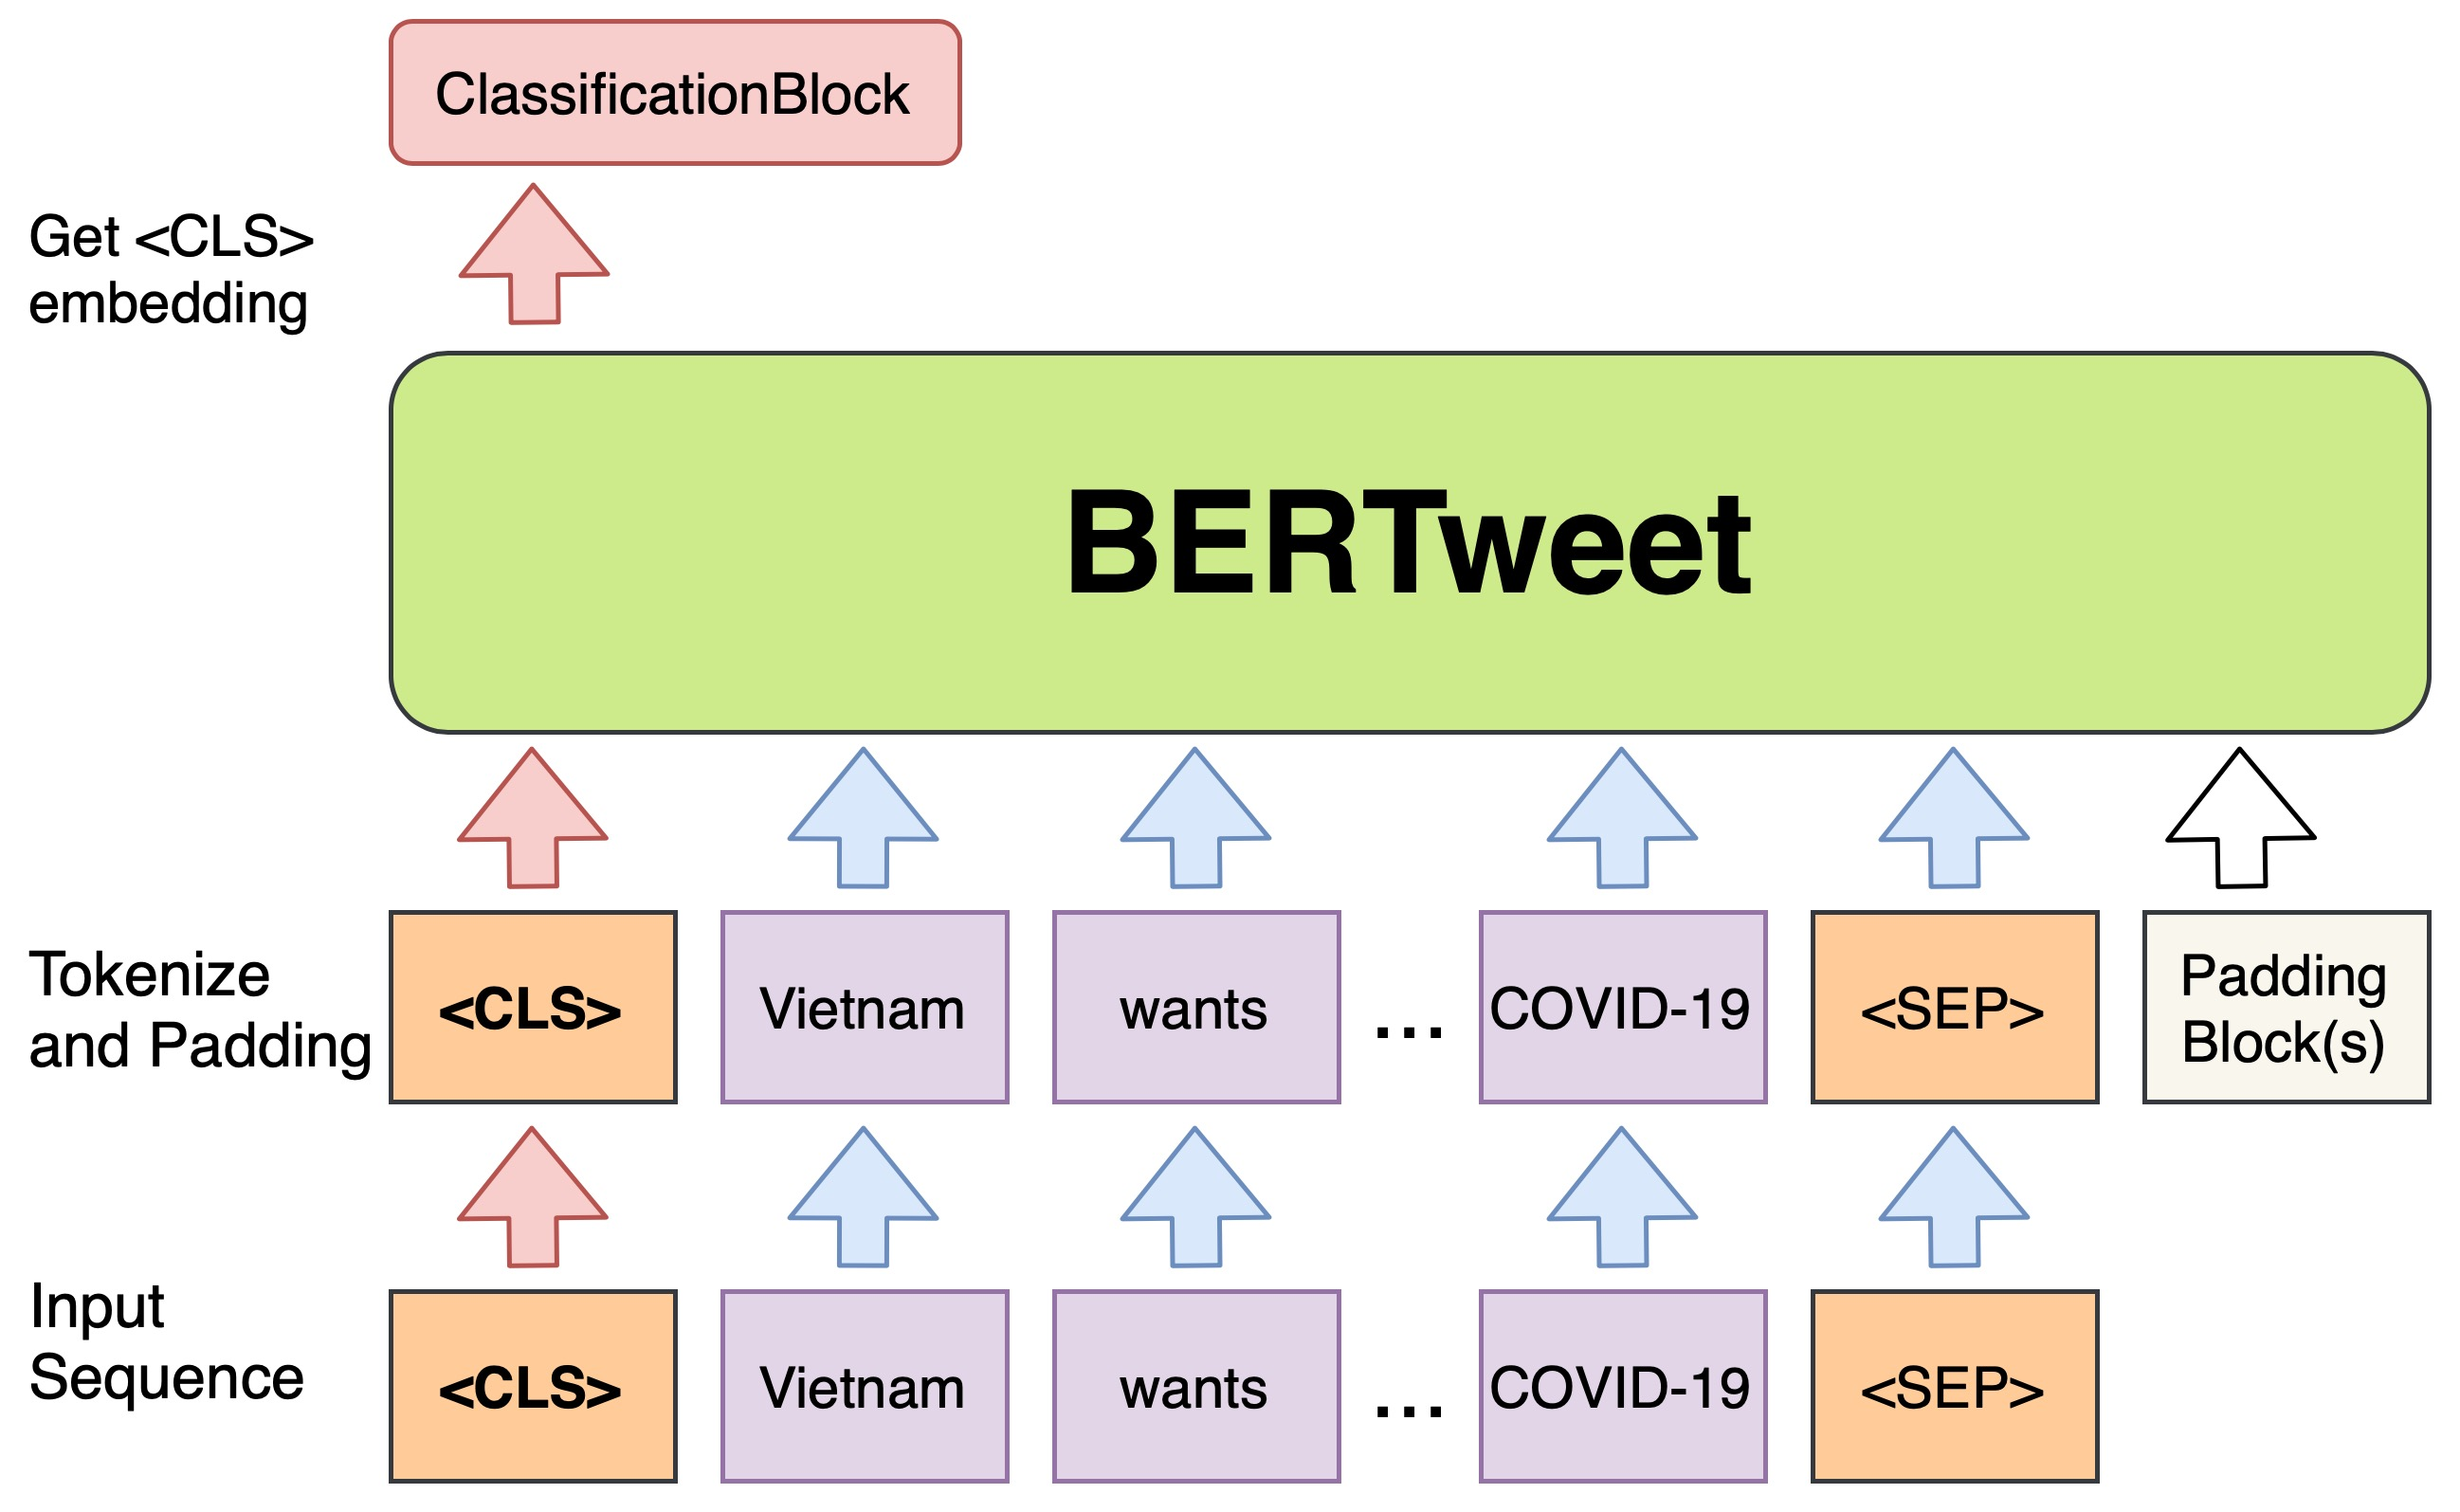
\includegraphics[width=\columnwidth]{Model.jpg}
    \caption{An overview of our model for identify Informative COVID-19 English Tweets}
    \label{fig:model}
\end{figure}

\subsection{BERTweet}
BERTweet \cite{BERTweet} is a large-scale language model pre-trained for English Tweets. Because of its nature of being a domain-specific model, BERTweet has achieved state-of-the-art performances on many downstream Tweet NLP tasks of Part-of-speech tagging, Named entity recognition and text classification, outperformed top models such as RoBERTa-base \cite{1907.11692} and XLM-R-base \cite{1911.02116}. Trained on 845M Tweets streamed from 01/2012 to 08/2019 and 5M Tweets related the COVID-19 pandemic as pre-training resources, BERTweet has an advantage compares to other models for our particular task of classifying COVID-19 related English Tweets.

\subsubsection{Embedding Extractions}
Each Transformer layer learns different information. We experiments different ways of extracting the pooled token from our BERTweet model to analyze the performance on this downstream task. More detail would be discussed in the ``Experiments'' section.

\subsubsection{Global Local BERTweet}
Due to the informal nature of writing Tweets, many tweets have noteworthy information at particular part of the tweets. Therefore, besides reading the whole Tweets, paying more attention to local parts of the Tweets is also important. Inspired by that idea, we propose a method to concurrently training 3 BERTweet models: one for reading the whole sequence, one for reading the first part of the sequence, and one for reading the remaining part. The pooled token from each model would then extracted and concatenated together for the system to learn both global and local information of the Tweets.

\subsection{Classification Block}
The classification block contains one or more linear layers stacked onto each other. The final layer is then used to classify whether a Tweet is informative or not.

\section{Experiments}
\subsection{Datasets}
We use the Dataset released by the competition organizer, consisting of 10,000 COVID-19 English Tweet. Each Tweet in the dataset is annotated by 3 annotators independently, and the overall inter-annotator agreement score of Fleiss' Kappa is 0.818. The dataset is then divided into 3 distinct set for training, validation, and testing, with the ratio of 70/10/20, respectively.

Table 1 shows the division of the dataset.

\begin{table}
    \centering
    \begin{tabular}{|c|c|c|}
        \hline
         & \bf{Informative} & \bf{Uninformative} \\ \hline
        Training Set & 3303 & 3697 \\ \hline
        Validation Set & 472 & 528 \\ \hline
        Test Set & 944 & 1056 \\ \hline
    \end{tabular}
    \caption{Dataset}
    \label{tab:Dataset}
\end{table}

\subsubsection{Re-splitting Data}
During the Evaluation Phrase, we re-splitting our dataset by combining Training and Validation sets then dividing randomly with the ratio of 90/10.

Table 2 shows the division of the dataset (not including the Test set).
\begin{table}
    \centering
    \begin{tabular}{|c|c|c|}
        \hline
         & \bf{Informative} & \bf{Uninformative} \\ \hline
        Training Set & ... & ... \\ \hline
        Validation Set & ... & ... \\ \hline
    \end{tabular}
    \caption{Dataset}
    \label{tab:Dataset}
\end{table}

\subsection{Implementation}
\subsubsection{Main Library and Framework}
We use the \texttt{transformers} library \cite{1910.03771} with \texttt{PyTorch} framework \cite{paszke2017automatic} to run our codes.

\subsubsection{Two-Phrases Training}
During Training progress, we follow the Two-phrases training, in which we freeze all BERTweet parameters during the first phrase and start with high learning rate to focus on training the Classification block. Because the Classification block is a combination of Linear layers, the training stage only takes a small amount of time to reach convergence.

\subsubsection{Optimizer}
Phuong: ADAM.

\subsubsection{Hyperparameters Configuration}
By examining the dataset, we observe that the longest sequence in the dataset has 89 words and 110 tokens (VERIFY). Therefore, we set the max length for padding and truncating before feeding into the BERTweet model to be 256, which helps decreasing training time and memory used.

We train our models on 1 NVIDIA DGX V100 and 1 NVIDIA RTX 2080. To fit the machine, we alternatively use batch size of 16 and 32.

Phuong: Within the Two-phrase training that we have discussed above, we use 10-12 epochs to train the classification block with the learning rate of $5^{-4}$ and 4-6 epochs to finetune the whole system with the learning rate of $10^{-5}$.


\subsection{Model Performance}
\subsubsection{Baselines}
Phuong
\subsubsection{BERTweet with different embedding selections}
We experiment different ways to extract embedding from the Transformer model. Table 3 shows the evaluation of these implementation.

The reported results are the F1 Score of predictions on the original validation set.
\begin{table}
    \centering
    \begin{tabular}{|c|c|}
        \hline
        Model & F1 \\\hline
        1 & 0.9028 \\\hline
    \end{tabular}
    \caption{Caption}
    \label{tab:my_label}
\end{table}

\subsubsection{Ensembling}
Phuong

\subsection{Additional Works}
...



\section{Future work}

\section{Conclusion}

PHUONG




\bibliographystyle{acl_natbib}
\bibliography{citation}

\end{document}
